\chapter{Introduction and Background}
Redundant, accurate flight vehicle localization has been well-documented over several decades~\cite{zhaoCooperativeLocalizationBased2017,rufaSensorFusionUnmanned2014,tennyRobustNavigationUrban2022,kandemirProbabilisticMeasurementMethod2018}. However, as the threat to GPS signals continues to rise, the need for robust positioning estimation increases. While robust systems already exist to combat incoming interference, these systems are either proprietary or government controlled, making them infeasible for widespread use. Cheaper, robust systems are critical for the safe future of civilian and military flight vehicles. Civilian aircraft feature a wide sensor suite the work in tandem to provide redundancy and safety critical features to maintain safe flight. These aircraft have the space to fit these sensors and the power to run them consistently in all phases of flight (Figure~\ref{fig:weights}), more importantly, the companies that design and build these aircraft also the budget to afford such expensive sensor suites.

\begin{figure}[!ht]\label{fig:weights}
    \centering
    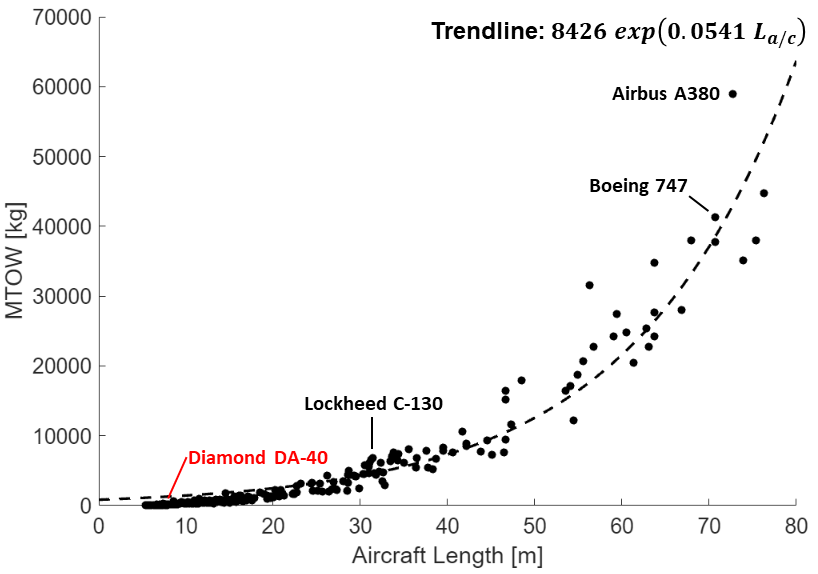
\includegraphics[width=.6\linewidth]{Figures/weights.png}
    \caption{Aircraft with a larger Max Takeoff Operating Weight (MTOW) typically have more space for more complex sensor suites compared to their General Aviation counterparts~\cite{AircraftCharacteristicsDatabase}.}
\end{figure}

Smaller aircraft are not allowed these luxuries, being manufactured with fewer sensors, overall making them less safe. Table~\ref{tbl:sensorsuitecomparison} compares the different sensors onboard a civilian airliner and a civilian general aviation aircraft.

\begin{table}[!ht]\label{tbl:sensorsuitecomparison}
    \caption{Inexhaustive list of sensors available to commercial and general aviation aircraft. (Adapted from~\cite{DiamondAircraftDA40,customerservicesA380AircraftCharacteristics2020})}
    \centering
    \begin{tabular}{lcc}
        \toprule
        \textbf{Sensor}                    & \textbf{Commercial} & \textbf{General Aviation} \\
        \midrule
        Pitot Tubes                        & \(5\)               & \(2\)                     \\
        Distance Measuring Equipment       & \(2\)               & \(1\)                     \\
        Ultra-High Frequency Sensors       & \(2\)               & \(1\)                     \\
        Very-High Frequency Sensors        & \(3\)               & \(2\)                     \\
        Communication Channels             & \(2\)               & \(2\)                     \\
        Outside Air Temperature Sensors    & \(4\)               & \(1\)                     \\
        Fuel Flow Gauge                    & \(4\)               & \(1\)                     \\
        GPS receivers                      & \(2\)               & \(1\)                     \\
        Inertial Measurement Units         & \(3\)               & \(1\)                     \\
        Satellite Communications           & \(1\)               & {--}                      \\
        Specific Impulse Sensors           & \(6\)               & {--}                      \\
        Weather Radar                      & \(1\)               & {--}                      \\
        Traffic Collision Avoidance System & \(4\)               & {--}                      \\
        Radio Altimeter                    & \(3\)               & {--}                      \\

        \bottomrule
    \end{tabular}
\end{table}

Regardless of size, the sensor suite aboard any flight vehicle is able to provide measurements 50 times greater than that of a GPS receiver, so a sensor fusion algorithm is optimal for this situation. Because sensor measurements have inherit errors due to a variety of factors, they can wander or \textit{dead reckon} through time. GPS measurements, although slower, provide measurements that do not drift at cost of being slightly less accurate. Table~\ref{tbl:sensorfusionframeworks} describes the most common sensor fusion frameworks for GPS and INS platforms.
\begin{table}[!ht]\label{tbl:sensorfusionframeworks}
    \caption{Common sensor fusion frameworks used for GPS and INS collection platforms}
    \centering
    \begin{tabular}{clc}
        \toprule
        \textbf{Name}            & \textbf{Level of Measurement}          & \textbf{Typical Error} \\
        \midrule
        \textit{Loosely-Coupled} & GPS Position and Velocity              & \(1~-~3\) [m]          \\
        \textit{Tightly-Coupled} & GPS Pseudorange and Doppler            & \(1~-~2\) [m]          \\
        \textit{Deeply-Coupled}  & GPS Inphase and Quadrature Correlators & \(\leq0.5\) [m]        \\
        \bottomrule
    \end{tabular}
\end{table}
This work presents a deeply-coupled sensor fusion algorithm known as vector tracking. Of the 3 types of GPS and INS sensor fusion frameworks, it is well-documented that deeply coupled provides the most accurate localization between measurement updates~\cite{wattsGPSGLONASSL12019}.
\section{Prior Art}
The objective of this thesis is to investigate the efficacy of position estimation for a flight vehicle in GPS-degraded and GPS-denied conditions. This thesis will analyze the performance through use of a deeply-coupled sensor fusion algorithm utilizing both INS and GPS measurements. The idea of fusing INS measurements and GPS measurements together on a flight vehicle is well-documented. The following subsections scratch the surface of work performed by other authors and their contributions to the field.
\subsection{Sensor Fusion Overview and Variation}
Sensor fusion between GPS and other sensors aboard flight vehicles has existed for years and continues to be developed. A precise, accurate, and robust navigation solution is achievable when redundant, expensive, and high-quality sensor are installed. More information about the sensors found aboard commercial aircraft and smaller aircraft can be found in~\cite{airbuscustomerservicesAirbusA380Aircraft2020} and~\cite{DiamondAircraftDA40}, respectively. Salmon~\cite{salmonExperimentalExplorationLowCost2015} provides an exploratory analysis using ground vehicles and their sensors complimented with a Ground Vehicle Dynamic Model (GVDM) in a tightly-coupled GPS/INS/GVDM sensor fusion. 

\subsection{Vehicle Dynamic Model Sensor Fusion}


\subsection{Other Types of Flight Vehicle Sensor Fusion}

\section{Field Contributions}
The focus of the research presented in this thesis is the performance evaluation of localization in GPS-degraded and GPS denied environments for simulated low-cost sensors aboard a small general aviation fixed wing flight vehicle. Taking that into consideration, the following contributions to the field are made:
\begin{itemize}
    \item Determination of the optimal flight vehicle model to use in the navigation algorithm when considering complexity and computational performance.
    \item Comparative analysis of multiple flight scenarios reflecting realistic flight plans and GPS degradation.
    \item Analysis of deeply-coupled sensor fusion algorithm using the flight vehicle model and simulated GPS measurements to determine the efficacy of safe localization in a real-life scenario.
\end{itemize}

\section{Thesis Outline}
The rest of this work follows a description of the physical systems simulated and modeled in the FVDM, satellited simulator, and GPS receiver. After, a presentation of the results, coupled with a Monte-Carlo analysis as a performance evaluation are shown. Wrapping up, final conclusion about the investigation are made and future work considerations are presented.